\documentclass[%
aip,
jmp,
reprint,
]{revtex4-1}

\usepackage{graphicx}% Include figure files
\usepackage{dcolumn}% Align table columns on decimal point
\usepackage{bm}% bold math
\usepackage{float}
\usepackage{siunitx}
\usepackage{hyperref}
\usepackage{listings}
%\usepackage[style=phys]{biblatex}
%\addbibresource{refs.bib}
\usepackage{ gensymb }
%\usepackage[mathlines]{lineno}% Enable numbering of text and display math
%\linenumbers\relax % Commence numbering lines
\usepackage{subcaption}
\usepackage{color}

\definecolor{dkgreen}{rgb}{0,0.6,0}
\definecolor{gray}{rgb}{0.5,0.5,0.5}
\definecolor{mauve}{rgb}{0.58,0,0.82}

\lstset{
	frame=tb, 
	language=Python, 
	columns=flexible,
	basicstyle={\small\ttfamily},
	keywordstyle=\color{blue},
	commentstyle=\color{dkgreen},
	stringstyle=\color{red},}

\mathchardef\mhyphen="2D

\renewcommand{\arraystretch}{1.3} % Changes the height of tables
\DeclareSIUnit\year{yr}
\DeclareSIUnit\parsec{pc}



\begin{document}
	
	\title[Short title]{Title}
	
	\author{Lucas, Miles}
	\author{Brandon, John}
	\affiliation{Iowa State University}
	
	\date{30 August 2017}
	
	
% Write here a short abstract (1 paragraph) describing what you achieved in this lab.

	\begin{abstract}
	
	Abstract will go here.
		
	\end{abstract}
	
	\maketitle
%________________________________________________________________________
	
%	Write here a summary of the goals of this lab. Be brief – do not exceed the end of the first page.

	\section{Introduction}
	
	
%________________________________________________________________________	

%	Describe your telescope and camera setup. For the first lab you should describe the setup in more details. Subsequent labs can refer to the procedure described in the first lab, and focus more on the data acquisition itself. Important details to write include: which stars have been observed, which filters were used (BVI), what exposure times and what calibration procedures have been followed (e.g., dark frames acquisition, photometric standards observed, etc.). Mention also the observing conditions (weather, moon presence, temperature, etc.). You should include the observing log appendix A (a table or a scan of a hardcopy). This section can be as long as necessary, but you should strive for brevity (you can refer to the lab guide to avoid repeating all steps, but make sure you explain anything you did differently, problems encountered, etc.). Use tables to summarize information clearly.

	\section{Data Acquisition and Setup}
	Observations were made on \date{30 August 2017} at the Zaffarano Hall observation deck in Ames, Iowa. The night was very clear and the ambient temperature was around \SI{32}{\degreeCelsius}. Observations were made using a Meade 8" reflector telescope with an SBIG ST-402ME CCD camera with internal V, B, and I filters. 
	
	To setup the telescope we used the Meade's GPS functionality to automatically calibrate its position. This calibration involved using two point sources as guides and orienting the telescope centered on the point source. For these measurements, the calibration sources were Arcturus and Altair. We used a \SI{32}{\milli\meter} eyepiece for our calibration alignment. Using the Meade selector, we navigated to the $\beta$ Cygni system We then switched to a \SI{9}{\milli\meter} eyepiece for fine-alignment on our target. Once we were well centered on our target we removed the eyepiece and inserted our CCD camera.
	
	Using CCDops we selected the V filter and began focusing the CCD camera with a manual knob on the telescope. The exposure time for these focusing grabs was \SI{0.05}{\second}. We based our focus on maximizing the peak amplitude read out in CCDops. We took multiple images at multiple exposures with different filters, all recorded in \autoref{table:log}. For each image grab, we set up an autograb using CCDops and took the frames. At each exposure level, we also took dark frames using autograb in order to reduce systematic error.
%________________________________________________________________________

%Describe what you did to analyze the data. For the first lab this section will be minimal. For subsequent labs you should describe in detail the steps you did to analyze the data.  If applicable you can attach the code you used to analyze the data in Appendix B (either a log of your IDL section, or the code of any scripts you wrote). You can also attach screenshots of your computer session if it helps your discussion. Include tables of raw data in this section. The goal of this section is to describe unambiguously what you did to derive your final images and measured quantities from the raw data. Again be brief but complete (use as much space as you need).
	\section{Data Analysis}
	
	Our analysis included some simple image processing and then used machine learning to determine the pixel scale and field of view. 
	
	Our processing pipeline involved finding median dark frames for each exposure length and then subtracting the dark frames from each science image. We use median dark frames rather than mean because we wanted to avoid outliers in the form of cosmic rays or dark pulses. To create the median images, we used a python script that utilizes numpy's array operations for getting the median of the data arrays from each FITS file. Once we saved the three median dark frames (\SI{0.1}{\second}, \SI{0.5}{\second}, \SI{1.0}{\second}) we used AstroImageJ to automate the subtraction for the 26 science images. A comparison of the science images before and after subtraction is shown in \autoref{fig:comparison}. As you can see, the thermal excitation caused by the camera's electronics is removed. 
	
	To calculate the pixel scale of our image, we need to find the center of each star. 
	
	\begin{figure}[]
		\begin{subfigure}{\linewidth}
			\centering
			
\includegraphics[width=.8\linewidth]{pre.png}
			\caption{Raw science image}
		\end{subfigure}
		\begin{subfigure}{\linewidth}
			\centering
			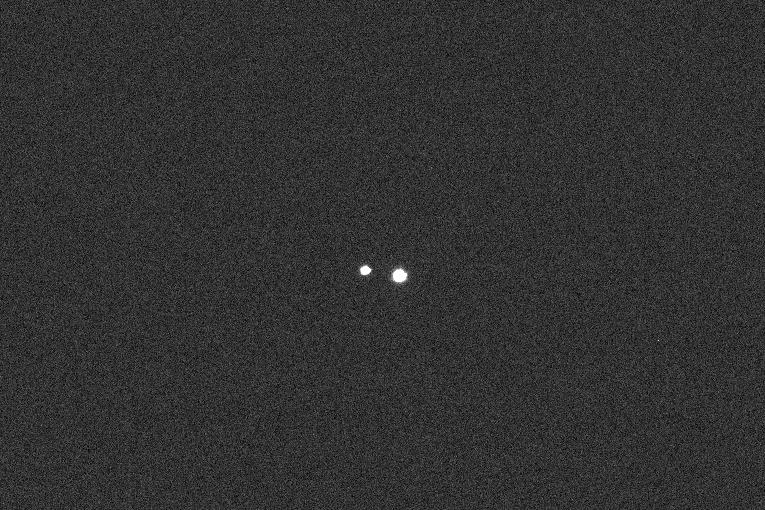
\includegraphics[width=.8\linewidth]{post.png}
			\caption{Processed science image}
		\end{subfigure}
		\caption{Comparison of the raw and processed science images of Albireo in photometric V at \SI{0.1}{\second} exposure.}
		\label{fig:comparison}
	\end{figure}
	
	


%________________________________________________________________________
	
%	Describe in detail the results you obtained from the quantitative analysis of your data, as explained in the lab guide.
	\section{Results}
	 
	
%________________________________________________________________________
	
%	Add here anything else you want to say, and summarize your results. This section should be very brief, not more than a couple of paragraphs
	\section{Conclusions}
	
	
%________________________________________________________________________
	
	\section*{Acknowledgements}
	
	Thank you to Dr. Charles Kerton and Brandon Marshall for their guidance and assistance in this work.
	
%	\printbibliography
	
	
%________________________________________________________________________
	
	\onecolumngrid
	\appendix
	\section{Observation Log}
	
	\begin{table}[h!]
		\centering
		\label{table:log}
		\caption{Observed 06 September 2017 by Miles Lucas and John Brandon}
\begin{tabular}{clclcccl}
	\hline
	Time  & File                   & N Frames & Object                                     & Filter &     Exposure     &       Camera Temp.        & Notes       \\ \hline\hline
	21:39 & M39\_2\_V\_13s\_       &    5     & M39 Objects x1, x4, x7, and x9; stars E, D &   V    & \SI{13}{\second} & \SI{5.33}{\degreeCelsius} &             \\
	21:41 & M39\_2\_V\_13s\_dark\_ &    5     & M39 Objects x1, x4, x7, and x9; stars E, D &   V    & \SI{13}{\second} & \SI{5.33}{\degreeCelsius} & Dark frames \\
	21:43 & M39\_2\_B\_13s\_       &    5     & M39 Objects x1, x4, x7, and x9; stars E, D &   B    & \SI{13}{\second} & \SI{5.33}{\degreeCelsius} &             \\ \hline
\end{tabular}

	\end{table}
%________________________________________________________________________
	
	\section{Analysis Scripts}
	
	File: lab2/src/measurements.py
	\lstinputlisting{../src/measurements.py}
	

\end{document}
%
% ****** End of file aipsamp.tex ******
